\documentclass[11pt]{article}

\usepackage[margin=1in]{geometry}
\usepackage{amsmath,amssymb}
\usepackage{booktabs}
\usepackage{tabularx}
\usepackage{threeparttable}
\usepackage{graphicx}
\usepackage{microtype}
\usepackage[
  backend=biber,
  style=apa,
  natbib=true,
  sorting=nyt,
  sortcites=true,
  maxbibnames=20
]{biblatex}
\addbibresource{references.bib}
\usepackage{siunitx}
\usepackage{caption}
\usepackage{subcaption}
\usepackage{enumitem}
\usepackage{float}
\usepackage{xcolor}
\usepackage[hidelinks]{hyperref}

\graphicspath{{figures/}}
\captionsetup{font=small,labelfont=bf}
\setlist{nosep,leftmargin=*}
\setlength{\parskip}{0.42em}
\setlength{\parindent}{0pt}
\newcommand{\code}[1]{\texttt{#1}}
% LaTeX 2025 makes \input robust; use the primitive form for generated row
% fragments so booktabs rules remain correctly aligned.
\makeatletter
\newcommand{\tableinput}[1]{\@@input{#1}}
\makeatother
\newcommand{\OneWeekForecast}{12,932}
\newcommand{\OneWeekLower}{11,836}
\newcommand{\OneWeekUpper}{14,028}
\newcommand{\JointWeeks}{101}
\newcommand{\ForecastWAPE}{9.8\%}
\newcommand{\ForecastCoverage}{85.6\%}


\title{From forecasts to reserves: Decision-focused evaluation of weekly dengue admissions in Bangladesh under potentially capacity-censored surveillance}
\author{
Abid Shahriyar\textsuperscript{a,*}\qquad
Farzana Momtaz Mithila\textsuperscript{b}\\[0.7em]
\small \textsuperscript{a}Advanced Manufacturing Group, 6B, Niharika Concord Tower, House \#138, Road \#4,\\
\small Kamal Ataturk Avenue, Block C, Banani, Dhaka 1213, Bangladesh\\
\small \textsuperscript{b}American International University--Bangladesh, 408/1 (Old KA 66/1), Kuratoli,\\
\small Khilkhet, Dhaka 1229, Bangladesh\\[0.35em]
\small
\begin{tabular}{@{}rl@{}}
E-mail: & \href{mailto:abidshahriyar954@gmail.com}{abidshahriyar954@gmail.com} (A. Shahriyar; corresponding author)\\
        & \href{mailto:farzana.mithila@aiub.edu}{farzana.mithila@aiub.edu} (F. M. Mithila)
\end{tabular}
}
\date{}

\begin{document}
\maketitle

\begin{abstract}
\textbf{Background:} By 15 October 2026, the Bangladesh Directorate General of Health Services had recorded 107,259 dengue hospital admissions and 331 deaths during 2026. Because high-frequency surveillance records admissions rather than total infections or admission-eligible demand, it may be capacity-censored. We evaluated forecast and allocation claims supportable under these constraints.

\textbf{Methods:} Public surveillance was harmonized to Sunday--Saturday weeks and combined with lagged point-weather proxies; outcomes were neither interpolated nor downscaled from monthly totals. Ten statistical and machine-learning models, including damped Holt, histogram gradient boosting (HGB), an ensemble, and biology-informed variants, were compared at one-, two-, and four-week horizons using expanding-window hindcasts and sequential conformal intervals. The selected one-week forecast was propagated through divisional allocation policies over \JointWeeks\ matched weeks, with HGB, a prospective rolling selector, and direct divisional forecasts as sensitivity analyses. Fixed and adaptive reserves were matched by total allocated units divided by total observed admissions; partial-identification scenarios varied unobserved demand.

\textbf{Results:} The equally weighted log-growth--HGB ensemble achieved one-week mean absolute error (MAE) of 226.5 and weighted absolute percentage error (WAPE) of \ForecastWAPE, improving MAE over HGB by 71.8 admissions (95\% block-bootstrap interval 9.2--149.5); nominal 80\% interval coverage was \ForecastCoverage. Biology constraints did not reliably improve accuracy. Ensemble forecasts with pooled divisional shares produced 14.5\% mean weekly shortage, 11.1\% admissions-weighted shortage, and 307 admission-equivalent shortfalls per week, while total allocation was 96.8\% of observed admissions. The observed-total oracle reduced mean shortage by 5.67 percentage points (95\% interval 3.08--8.36). At aggregate-matched budgets, adaptive rules reduced unweighted shortage, but weighted and surge benefits were absent or uncertain; annual all-cause occupancy offered no stable allocation benefit.

\textbf{Conclusions:} Weekly forecasting of reported dengue admissions is workable for national preparedness, but performance did not justify enforcing biological constraints. The ensemble result requires prospective validation because it was identified in the completed hindcast. The defensible resource result is a decision-linked reserve frontier under potentially censored surveillance, not an estimate of unmet demand or exact physical resources.
\end{abstract}

\noindent\textbf{Keywords:} dengue; Bangladesh; infectious disease forecasting; decision analysis; resource allocation; partial identification

\section{Introduction}

Dengue is a climate-sensitive mosquito-borne infection whose expanding burden increasingly tests surveillance and hospital preparedness. Bangladesh has shifted from episodic, predominantly urban outbreaks toward recurrent and geographically dispersed transmission, and the 2023 epidemic demonstrated the scale at which reported admissions can stress the health system \citep{hasan2024,bhowmik2026,whoSitrep2023}. The pressure remains immediate: from 1 January through 15 October 2026, DGHS recorded 107,259 dengue hospital admissions and 331 deaths \citep{dghsDashboard}. For a planner, however, the actionable question is not simply whether dengue will increase. It is how much capacity to prepare, where to place it, and how to act when both the forecast and the observed demand signal are incomplete.

The forecasting and resource decisions are linked but not identical. A model may have favorable average error yet fail during outbreak growth, produce poorly calibrated uncertainty, or induce a costly allocation when translated across locations. Conversely, a slightly less accurate point forecast may support a safer decision if its uncertainty is well characterized. This distinction is especially important in Bangladesh because the routinely available high-frequency outcome is reported hospital admission. It does not enumerate all infections, all symptomatic presentations, or people refused, diverted, waitlisted, transferred, or treated outside reporting facilities. During congestion, reported admissions may therefore reflect both disease transmission and the capacity of the observation system.

This study evaluates a complete forecast-to-reserve chain while limiting its claims to quantities identified by the available data. We ask four questions: (i) how accurately can reported national admissions be forecast one to four weeks ahead under leakage-safe rolling evaluation; (ii) do biologically motivated weather lags and shape constraints improve forecasts beyond simple and flexible baselines; (iii) how do national forecast error, uncertainty reserves, and recent divisional shares translate into shortage and unused allocation; and (iv) are allocation conclusions robust when reported admissions are only a possible lower bound on admission-eligible demand?

The contribution is not a new claim that weather predicts dengue or that machine learning should replace conventional time-series baselines. Rather, it is a decision-focused evaluation that connects an auditable weekly target, strong time-series comparators and a simple ensemble, probabilistic planning intervals, exact aggregate-budget-matched allocation comparisons, and partial identification of unobserved demand. Figure~\ref{fig:workflow} summarizes that chain.

\begin{figure}[H]
\centering
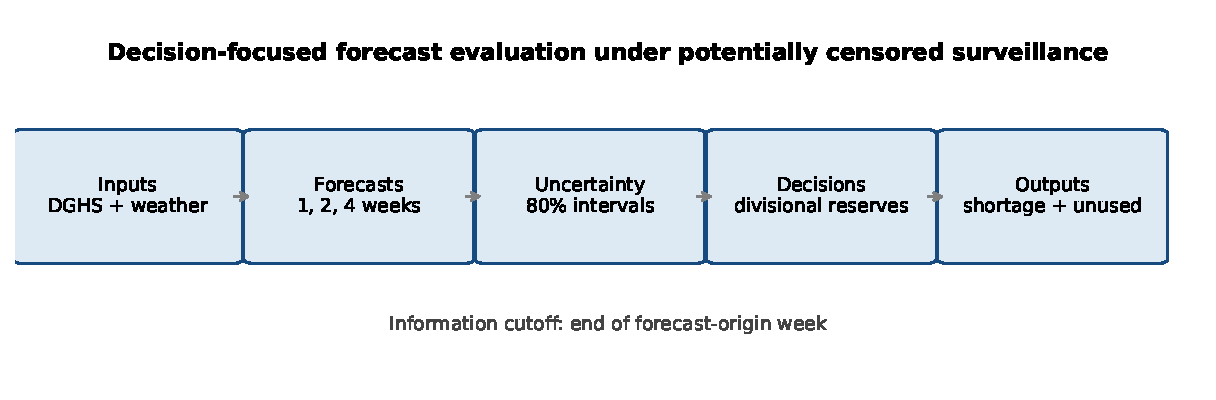
\includegraphics[width=0.98\textwidth]{study_workflow.pdf}
\caption{Study workflow. Every historical forecast uses only information available at its origin; allocation policies are then evaluated against subsequently reported divisional admissions and declared latent-demand scenarios.}
\label{fig:workflow}
\end{figure}

\section{Related work and research gap}

\subsection{Dengue forecasting: from climate associations to prospective prediction}

Dengue early-warning research spans seasonal autoregression, generalized linear models, climate-driven models, tree ensembles, neural networks, and mechanistic or hybrid approaches. Climate variables are epidemiologically plausible because rainfall can alter breeding habitat and temperature affects mosquito development, survival, biting, and viral replication. Yet plausibility does not guarantee incremental forecast value after recent cases and seasonality are known. In a prospective comparison for Mexico, climate-driven forecasts did not significantly improve on a seasonal autoregressive model, illustrating why added predictors must be judged out of sample rather than by in-sample association \citep{johansson2016}. Operational studies in Brazil and Vietnam further show that forecast value depends on lead time, season, geography, probabilistic calibration, and the decision deadline \citep{lowe2014,colon2021}.

Evaluation practice remains uneven. A systematic review of 64 studies covering 99 dengue prediction models found that approximately one fifth reported no validation and only 5.2\% used external validation; the review also identified inconsistent handling of lags, reporting processes, and model comparison \citep{leung2023}. The multi-team dengue forecasting challenge likewise emphasized common targets, genuinely out-of-sample assessment, probabilistic output, and relevance to public-health decisions rather than isolated accuracy claims \citep{johansson2019}. These findings motivate our use of repeated historical origins, common target weeks, simple baselines, interval scoring, season-specific results, and an explicit selection-bias sensitivity.

\subsection{Biological information and lag structure}

Mechanistic evidence supports a nonlinear rather than universally increasing temperature effect. Laboratory-informed transmission models place an approximate \textit{Aedes aegypti} dengue suitability window near 18--34\,$^\circ$C, with a peak in the high twenties; risk declines outside that window because individual mosquito and viral traits respond differently to temperature \citep{mordecai2017,ryan2019}. Rainfall is also non-monotone: it can create larval habitat but intense rain can flush immature mosquitoes. Weather effects should therefore be distributed across time, spanning habitat formation, mosquito development, extrinsic viral incubation, human incubation, symptom progression, care seeking, and hospitalization.

Most biology-informed prediction work nevertheless faces a tension between structural plausibility and predictive misspecification. A constraint can reduce implausible extrapolation, but it can also be wrong at the scale of aggregated observations when serotype, immunity, vector control, mobility, water storage, care seeking, and reporting are omitted. We therefore treat biological constraints as a falsifiable forecast hypothesis. They are retained only if they improve performance at future historical origins, rather than being assumed superior because they accord with mechanism.

\subsection{Bangladesh evidence}

Bangladesh studies have established long-run climate associations and increasingly used machine learning. El Ni\~no--Southern Oscillation and the Indian Ocean Dipole have been associated with dengue incidence \citep{banu2015}. More recent work has combined hospitalized cases with meteorological and socioeconomic data, applied feature-selection pipelines to meteorological predictors, and constructed interpretable tree-based early-warning systems using climate, sociodemographic, and landscape factors \citep{dey2022,mobin2024,rahman2025}. Other studies have compared regression, XGBoost, recurrent neural networks, and seasonal time-series models \citep{faruk2026}. A recent district-panel framework explicitly selected different models for tactical and strategic horizons and incorporated climate and serotype covariates \citep{fuad2026}.

This growing literature means that ``weather plus machine learning'' is no longer a sufficient novelty claim. Important operational gaps remain: reported cases or admissions are not always distinguished from infection incidence; daily records may be grouped into weeks without validating the reporting calendar; missing high-frequency outcomes can be silently interpolated; performance is often separated from forecast uncertainty and the downstream resource decision; and denied demand is unavailable precisely when capacity may bind. Our study addresses these gaps at the national-to-division planning interface.

\subsection{From forecast accuracy to allocation value}

Forecast evaluation metrics are not necessarily aligned with allocation loss. Allocation scoring rules can rank infectious-disease forecasts differently from generic probabilistic scores when locations compete for limited resources \citep{gerding2024}. Forecast-to-allocation systems have also been developed for collaborative health-resource planning and regime-aware outbreak response \citep{jiang2024,soto2026}. These studies establish the importance of evaluating the decision induced by a forecast, not merely the forecast itself.

Our scope is deliberately narrower than a full hospital optimization. We do not observe staffed beds, free beds, inventories, transfer limits, workforce availability, or patient-level length of stay. We therefore evaluate admissions-service-equivalent reserves and spatial policies, report shortage and unused allocation separately, compare adaptive rules with fixed reserves at equal ratios of total allocated units to total observed admissions, and avoid declaring an economically optimal reserve without verified cost functions.

Table~\ref{tab:literature} summarizes the established evidence and the specific gap addressed by this study.

\begin{table}[H]
\centering
\caption{Position of the present study within the dengue forecasting and decision literature.}
\label{tab:literature}
\begin{threeparttable}
\footnotesize
\begin{tabularx}{\textwidth}{@{}p{0.16\textwidth}p{0.21\textwidth}XX@{}}
\toprule
Literature stream & Representative evidence & What is established & Gap addressed here \\
\midrule
Forecast evaluation & \citet{leung2023,johansson2016,johansson2019} & Validation design, baselines, horizon, and probabilistic calibration can change conclusions. & Common-target expanding-window hindcasts, simple and ML baselines, intervals, season/intensity strata, and prior-origin selection sensitivity. \\
Operational climate forecasting & \citet{lowe2014,colon2021} & Climate-informed forecasts can support planning, but value varies by lead time and season. & Weekly Bangladesh admissions forecast tied directly to reserve decisions rather than climate association alone. \\
Biological mechanisms & \citet{mordecai2017,ryan2019} & Temperature suitability is unimodal; weather effects operate through distributed biological delays. & Explicit lagged suitability and heat-stress features, with prospective tests of monotonic constraints and permission for a negative result. \\
Bangladesh dengue models & \citet{banu2015,dey2022,mobin2024,rahman2025,faruk2026,fuad2026} & Autoregression, climate, socioeconomic factors, serotype, and ML can contribute to prediction. & Validated Sunday--Saturday admissions target, no synthetic weekly outcomes, forecast uncertainty, and downstream allocation scoring. \\
Decision-linked evaluation & \citet{gerding2024,jiang2024,soto2026} & Forecast rankings can change under allocation loss; adaptive preparedness can be optimized when costs and constraints are known. & Exact aggregate-budget-matched fixed versus adaptive reserves plus partial identification when true unmet demand and operational costs are unavailable. \\
\bottomrule
\end{tabularx}
\begin{tablenotes}
\footnotesize
\item The study's novelty lies in the combined design and the restricted claims supported by public data, not in introducing weather covariates or a new generic machine-learning architecture.
\end{tablenotes}
\end{threeparttable}
\end{table}

\section{Data and study design}

\subsection{Surveillance target and weekly calendar}

The primary source was the Bangladesh Directorate General of Health Services (DGHS) Health Emergency Operation Center dengue dashboard \citep{dghsDashboard}. It publishes national admission and death series and cross-sectional views by division or city corporation, age, and sex. The modeling outcome was reported hospitalized dengue admissions. This is an operational workload signal, not total symptomatic incidence: infections that do not present, outpatients, unreported facilities, and patients refused, diverted, waitlisted, or transferred are not comprehensively observed.

Daily surveillance and weather data were aggregated to the DGHS week, Sunday through Saturday. Week 1 is the Sunday--Saturday interval containing 1 January; thus 9--15 August 2026 is week 33. The week-year was retained separately from calendar year at year boundaries. Public endpoints were accessed with ordinary requests and cached by year. No access control or anti-bot mechanism was bypassed, and acquisition stops on malformed or unsuccessful responses.

\subsection{Historical dengue and environmental covariates}

Pre-2024 history was reconciled against the repository accompanying the Bangladesh review by \citet{bhowmik2026}, pinned to a source-control commit, and compared with OpenDengue version 1.3 \citep{clarke2024,opendengue2025}. Temporal resolution varies across years. Exact daily or weekly observations were eligible for high-frequency modeling; monthly totals were retained for context but never divided into synthetic weeks. The long 2020--2021 high-frequency gap was left missing.

Daily precipitation, mean, minimum and maximum temperature, and relative humidity came from the NASA POWER point API \citep{nasaPower}. Eight points represented the divisional capitals. These are transparent proxies, not population-weighted polygon averages. Variables were summarized within DGHS weeks and across available capital points, while missing-day fractions were retained for audit.

\subsection{Operational context and missing-data protocol}

Public DGHS facility pages supplied 2025 approved-bed counts and annual all-cause bed-occupancy rates. They do not measure staffed dengue beds or free capacity in a target week. A 2023 Transparency International Bangladesh report was used only to triangulate capacity pressure \citep{tib2023}. A 2019 cohort of 1,978 Group B/C patients in three Dhaka tertiary hospitals reported a median five-day stay and 4.5 L total intravenous-fluid use \citep{chowdhury2024}; these values support illustrations, not national clinical standards.

Missingness was classified before treatment \citep{little2019}. Structural absence and incomplete outcome weeks remained missing and were excluded from scoring. Predictor imputers, when required, were fitted inside each historical training fold; missingness indicators were retained where appropriate. We prohibited monthly-to-weekly allocation, interpolation of the 2020--2021 outcome blackout, full-series imputation before validation, evaluation against imputed outcomes, and two-sided smoothing in a prospective experiment. Table~\ref{tab:data} records the analytical role and excluded interpretation of each source.

\begin{table}[H]
\centering
\caption{Data sources, analytical roles, and interpretation boundaries.}
\label{tab:data}
\begin{threeparttable}
\small
\begin{tabularx}{\textwidth}{@{}p{0.20\textwidth}p{0.21\textwidth}X X@{}}
\toprule
Source & Resolution & Permitted use & Excluded interpretation \\
\midrule
DGHS dengue dashboard & Daily national; published weekly spatial summaries & Admission and death context, forecast target, historical divisional shares & Total infections or complete admission-eligible demand \\
Bhowmik et al. repository and OpenDengue & Source-dependent daily, weekly, or monthly history & Provenance reconciliation and eligible high-frequency history & Synthetic weekly values from monthly totals \\
NASA POWER & Daily point weather at eight capitals & Lagged weekly environmental proxy features & Population-weighted division-wide exposure \\
DGHS facility pages and TIB report & Annual public-facility context and selected outbreak snapshot & Sensitivity analysis and contextual evidence & Live staffed/free dengue beds or national denied demand \\
Dhaka Group B/C cohort & Patient cohort at three tertiary hospitals & Length-of-stay and fluid-use illustrations & National mean, prescription, or minimum resource standard \\
\bottomrule
\end{tabularx}
\end{threeparttable}
\end{table}

\section{Methods}

\subsection{Forecast estimand and expanding-window evaluation}

Let $Y_t$ be complete reported national dengue admissions in DGHS week $t$. At the end of week $t$, a model predicts $Y_{t+h}$ for $h\in\{1,2,4\}$. The experiment used expanding training windows and every eligible target from 2024 onward. At each origin, the training set ended early enough that the forecast target had already resolved; predictors and imputation parameters were restricted to information available at that origin. Hyperparameters were fixed across origins.

Ten primary models were compared: persistence; a trailing four-week mean; a 52-week seasonal naive model; a four-week log-count growth extrapolation; a regularized negative-binomial generalized linear model (NB-GLM); damped Holt exponential smoothing on the log-count scale; a baseline histogram gradient-boosting (HGB) model with Poisson loss; HGB with additional biological features; HGB with selected monotonic biological constraints; and an equally weighted log-growth--baseline-HGB ensemble. HGB was used because it accommodates nonlinear interactions and missing predictors without global preprocessing. Core models were scored on 124 common one-week targets. Damped Holt used 111 one-week targets because it required at least 12 observations in the most recent contiguous training segment; its smaller denominator is reported rather than filled.

Baseline HGB features included recent admissions and rolling summaries, cyclical week-of-year terms, a time index, and lagged precipitation, rainy days, temperature, and humidity. The log-growth model fitted a linear slope to $\log(1+Y)$ over the latest four complete weeks and extrapolated it by the required horizon. Damped Holt jointly selected level, trend, and damping parameters from a fixed grid using training-only one-step error. To repair the initially unstable NB-GLM, count lags and rolling means were transformed by $\log(1+x)$, only seasonal harmonics were retained as calendar terms, the linear time trend was removed, and stronger ridge regularization was used. The equally weighted ensemble averaged log-growth and baseline-HGB predictions without tuning the weight. The primary errors were mean absolute error (MAE), root mean squared error, and weighted absolute percentage error,
\begin{equation}
\mathrm{WAPE}=\frac{\sum_t|Y_t-\widehat{Y}_t|}{\sum_t Y_t}.
\end{equation}
Signed bias, peak-quartile error, interval coverage, interval width, and interval score were secondary outcomes.

The lowest-MAE model over the completed hindcast was labeled the \emph{best in backtest}, not a prospectively proven winner. To quantify model-selection optimism, a rolling selector chose among candidates using only earlier forecasts whose targets had resolved at each historical origin; before 20 resolved comparisons per candidate, baseline HGB was used. Performance was also stratified by target year and admission-intensity quartile. Paired model differences used 2,000 year-stratified moving-block bootstrap samples with four-week blocks.

\subsection{Biology-informed features and constraints}

Mechanistic evidence places a unimodal \textit{Aedes aegypti} dengue transmission window near 18--34\,$^\circ$C, with a peak in the high twenties \citep{mordecai2017,ryan2019}. We encoded a transparent triangular suitability score equal to zero at 17.8 and 34.6\,$^\circ$C and one at 29.1\,$^\circ$C. This was a forecasting approximation, not a reproduction of the full mechanistic $R_0(T)$ curve.

Distributed features at lags 0, 1, 2, 3, 4, 6, 8, 10 and 12 weeks included thermal suitability, the fraction of days within the thermal window, heat stress, heavy-rain frequency, and temperature--rain interactions. The lag span represents habitat formation and mosquito development, extrinsic viral incubation, human incubation (commonly about 4--10 days), symptom progression, care seeking, and hospitalization \citep{whoFacts}. Raw temperature and rainfall were not forced to increase admissions because both have defensible non-monotone effects. In the constrained sensitivity model, only engineered thermal suitability was constrained upward and heat stress downward, conditional on other predictors. The hypothesis was empirical: biological constraints would be retained only if they improved rolling-origin accuracy.

\subsection{Sequential planning intervals}

Locally scaled conformal intervals were constructed sequentially, inspired by conformal methods for dependent time series \citep{xu2021}. At origin $t$, only residuals from target weeks that had resolved were eligible. Absolute residuals were divided by $\sqrt{\widehat{Y}}$ to accommodate count heteroscedasticity; the empirical 80th percentile of the most recent 52 eligible scaled residuals was mapped back to the current forecast scale, followed by a transparent 10\% expansion of the radius. These are empirical planning intervals, not exact finite-sample guarantees under exchangeability. Coverage, mean width, and interval score were evaluated.

\subsection{Forecast-to-allocation policies}

Let $D_{it}$ be reported admissions in division $i$ and target week $t$, and let $B_t$ be the national allocation budget. The primary spatial policy used the pooled trailing three-week reported share,
\begin{equation}
\widehat{s}^{\mathrm{pool}}_{it}=
\frac{\sum_{k=1}^{3}D_{i,t-k}}
{\sum_j\sum_{k=1}^{3}D_{j,t-k}},
\qquad A_{it}=B_t\widehat{s}^{\mathrm{pool}}_{it}.
\end{equation}
Comparators used the latest share, the normalized maximum recent share, and a non-normalized maximum-share envelope. The envelope can exceed $B_t$ because each division receives its own recent maximum share; that excess is a spatial reserve premium.

The primary joint hindcast paired the best-in-backtest one-week national forecast with these shares over \JointWeeks\ target weeks having a calibrated interval and eligible spatial observations. The allocation was repeated with pre-specified baseline HGB and the prior-origin-only rolling selector to test dependence on hindsight model choice. A direct divisional baseline independently extrapolated the four-week log-count slope in each division and therefore bypassed national-to-division disaggregation; 99 weeks had the required four within-year history observations. An observed-total oracle replaced the forecast total by the realized divisional total, separating national forecast and aggregation error from spatial-share error. National budgets were then increased by fixed reserves from 0\% to 100\% in 5\% increments, by the upper 80\% interval bound, or by the spatial envelope.

The forecast and allocation denominators serve different purposes and are not a single nested cohort. Core one-week forecast models had 124 common scored targets. The selected ensemble yielded 128 point predictions, 108 of which had enough resolved residual history for a conformal interval. Of those 108, six W01--W03 targets in 2025--2026 lacked three prior within-year divisional weeks and the in-progress 2026 W41 spatial week was excluded, leaving \JointWeeks\ allocation targets. This accounts explicitly for the apparent 124-to-101 reduction.

Weekly aggregate shortage and unused allocation were
\begin{equation}
S_t=\frac{\sum_i\bigl(D_{it}-A_{it}\bigr)_{+}}{\sum_i D_{it}},
\qquad
U_t=\frac{\sum_i\bigl(A_{it}-D_{it}\bigr)_{+}}{\sum_i A_{it}}.
\end{equation}
We report the unweighted mean of $S_t$, shortage weighted by weekly admissions, absolute weekly and total admission-equivalent shortfalls, 90th-percentile shortage, unused allocation, worst-division service, and the fraction of weeks in which every division was covered. The primary budget measure was
\begin{equation}
R=\frac{\sum_t\sum_i A_{it}}{\sum_t\sum_i D_{it}},
\end{equation}
the ratio of total allocated units to total observed admissions; the mean of weekly budget ratios was retained only as a secondary diagnostic. Surge performance was defined on the top quartile of weekly divisional totals. Each adaptive policy was compared with an exact fixed-reserve rule having the same $R$. Paired differences in unweighted, admissions-weighted, and surge-week shortage used 2,000 year-stratified four-week moving-block bootstrap replicates. No policy was declared economically optimal because verified shortage, holding, expiry, transfer, and activation costs were unavailable.

\subsection{Potential capacity censoring and partial identification}

Reported admissions were treated as observed workload and a possible lower bound, not as an estimate of unconstrained need. Latent admission-eligible demand was represented as
\begin{equation}
L_{it}=D_{it}\{1+\delta g_{it}\},
\end{equation}
where $\delta\in\{0,0.25,0.50,1.00\}$ was the maximum proportional uplift and $g_{it}\in[0,1]$ specified a spatial pattern. Ten profiles were evaluated: uniform, linked to the normalized annual all-cause occupancy proxy, inversely linked, and seven rotations of the linked profile. Five national reserve levels (0, 25, 50, 75 and 100\%) and four spatial policies produced 800 profile-level combinations and 80,800 week-policy observations.

The occupancy proxy was deliberately weak: it was annual, all-cause, and did not measure staffed dengue capacity. Candidate weights between pooled reported shares and the proxy were evaluated using worst-profile shortage and worst-profile regret. The analysis asks whether a policy conclusion survives a declared identification region; it does not estimate the frequency or magnitude of refused or displaced demand.

\subsection{Reproducibility and reporting}

Acquisition, preprocessing, forecasting, interval construction, allocation, and stress testing were implemented as scripted stages with cached public inputs, machine-readable outputs, a source registry, and fixed seeds. The 4--10 October 2026 forecast-origin week contained seven published admission days; the 11--17 October target was generated only after that origin week closed. Reporting was informed by TRIPOD+AI where applicable to prediction-model development and evaluation \citep{collins2024}.

\section{Results}

\subsection{Forecast performance and uncertainty}

The equally weighted log-growth--HGB ensemble was the best-in-backtest point model at all three horizons (Table~\ref{tab:selected}). Its MAE was 226.5, 389.2, and 764.9 admissions at one, two, and four weeks, with corresponding WAPE of 9.8\%, 16.9\%, and 33.2\%. The sharp deterioration with horizon supports rolling weekly planning rather than treating a four-week forecast as equally actionable.

\begin{table}[H]
\centering
\caption{Best-in-backtest model by forecast horizon.}
\label{tab:selected}
\resizebox{\textwidth}{!}{%
\begin{tabular}{@{}llrrrrr@{}}
\toprule
Horizon & Model & $N$ & MAE & WAPE (\%) & Coverage (\%) & 2026 coverage (\%) \\
\midrule
\tableinput{tables/forecast_selected.tex}
\bottomrule
\end{tabular}}
\begin{minipage}{0.92\textwidth}
\footnotesize\emph{Note:} Models were selected descriptively by MAE over completed common-target hindcasts. Coverage refers to nominal 80\% sequential planning intervals and is unavailable at early origins until adequate residual history accumulates.
\end{minipage}
\end{table}

At one week, the ensemble MAE was 71.8 admissions lower than baseline HGB on 128 paired predictions (95\% year-stratified block-bootstrap interval $-149.5$ to $-9.2$); the estimated probability of lower MAE was 0.991. Its MAE was lower than baseline HGB separately in 2024, 2025, and 2026 (Table~\ref{tab:season}), but only three outbreak seasons were available and the ensemble was identified from the completed hindcast. The prior-origin-only rolling selector returned WAPE values of 10.6\%, 18.1\%, and 41.4\% at one, two, and four weeks, respectively. Thus, the prospective rule approached the ensemble at one and two weeks but not at four weeks; neither result substitutes for a genuinely frozen external-season evaluation.

\begin{table}[H]
\centering
\caption{One-week performance by target year for the ensemble and pre-specified baseline HGB.}
\label{tab:season}
\begin{tabular}{@{}llrrrr@{}}
\toprule
Year & Model & Weeks & MAE & WAPE (\%) & Mean bias \\
\midrule
\tableinput{tables/forecast_by_season.tex}
\bottomrule
\end{tabular}
\end{table}

For the one-week ensemble, WAPE was 8.5\% in the peak admission quartile and 30.2\% in the trough quartile. The difference reflects WAPE's small denominator during low-volume weeks; absolute errors were much larger at peaks. Its empirical 80\% interval coverage was \ForecastCoverage\ overall and 90.0\% in 2026. Figure~\ref{fig:backtest} displays predictions, intervals, and residuals by horizon.

\begin{figure}[H]
\centering
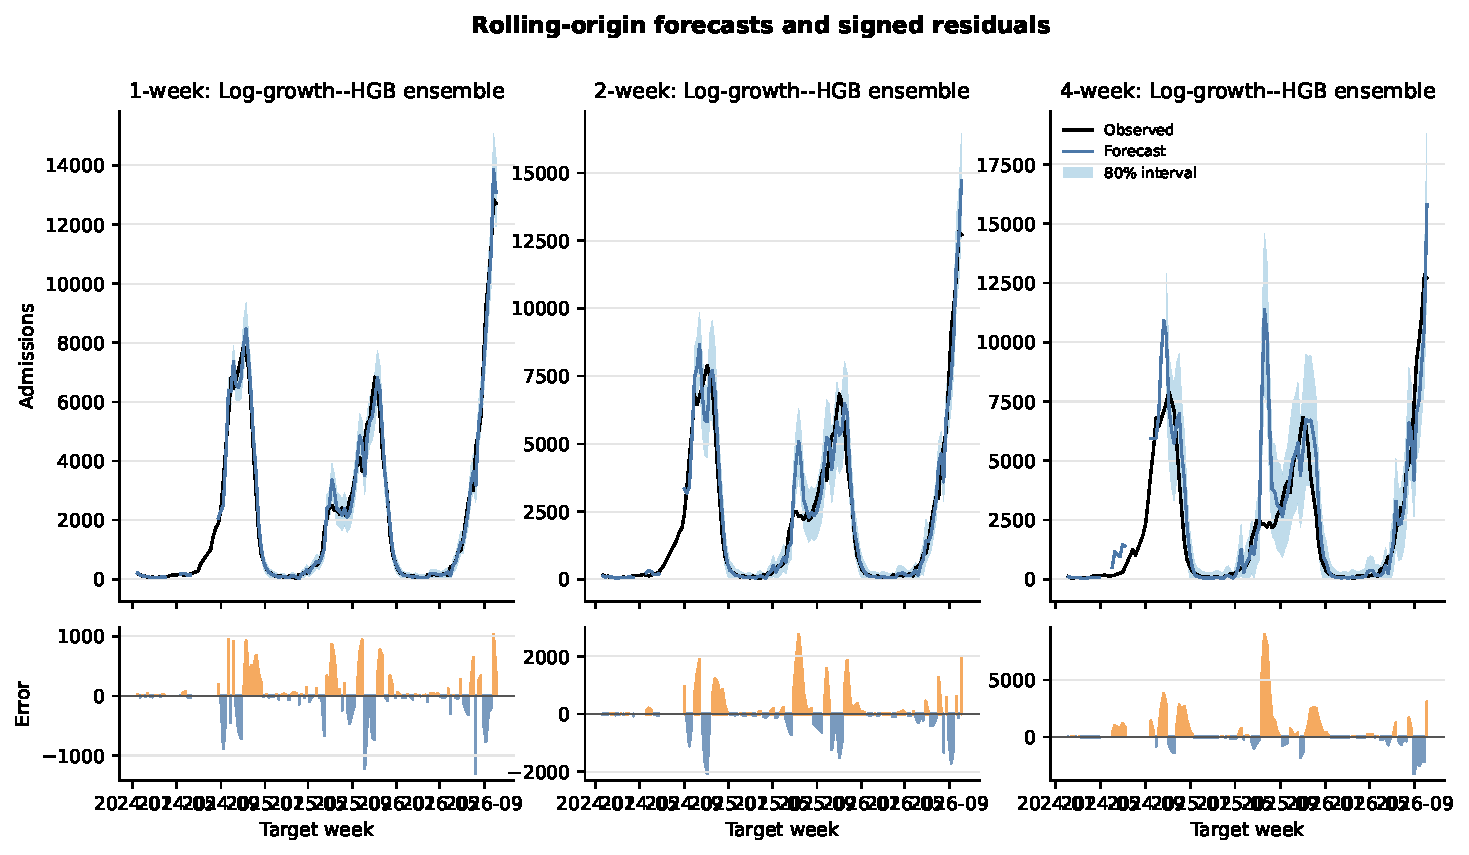
\includegraphics[width=0.98\textwidth]{forecast_backtest.pdf}
\caption{Expanding-window forecasts and residuals for the best-in-backtest model at each horizon. Shaded bands are sequential nominal 80\% planning intervals when enough resolved residuals were available.}
\label{fig:backtest}
\end{figure}

\subsection{Biology-informed forecasting as a negative result}

Adding biological features or constraints did not reliably improve forecast accuracy. At one week, baseline HGB MAE was 300.8, compared with 313.4 for biology-feature HGB and 312.6 for constrained biology HGB. At two weeks, baseline HGB remained best among the HGB variants. Although constrained biology HGB had a slightly lower four-week aggregate MAE (948.9 versus 951.5 for baseline HGB), the paired difference was $+30.1$ admissions and its 95\% interval ($-59.6$ to 145.6) did not support a gain. Differences between aggregate and paired estimates arise from model-specific eligible targets.

Figure~\ref{fig:performance} compares all primary models by MAE skill relative to persistence. Removing the linear time trend and using log-lags stabilized the NB-GLM, but its one-week MAE was 438.0, 25.7\% worse than persistence. Damped Holt was competitive (MAE 265.2) on 111 eligible one-week targets, while the ensemble combined the positive outbreak-growth response of log-growth with HGB's tendency to shrink extremes. The biology result should not be read as evidence that biology is irrelevant. Recent admissions may already compress transmission state at one week, and capital-point weather may be too coarse to add independent signal. It does show that biological plausibility alone is insufficient reason to impose a constraint on the operational forecast.

The complete model comparison, including probabilistic performance, is reported in Table~\ref{tab:forecastfull}.

\begin{figure}[H]
\centering
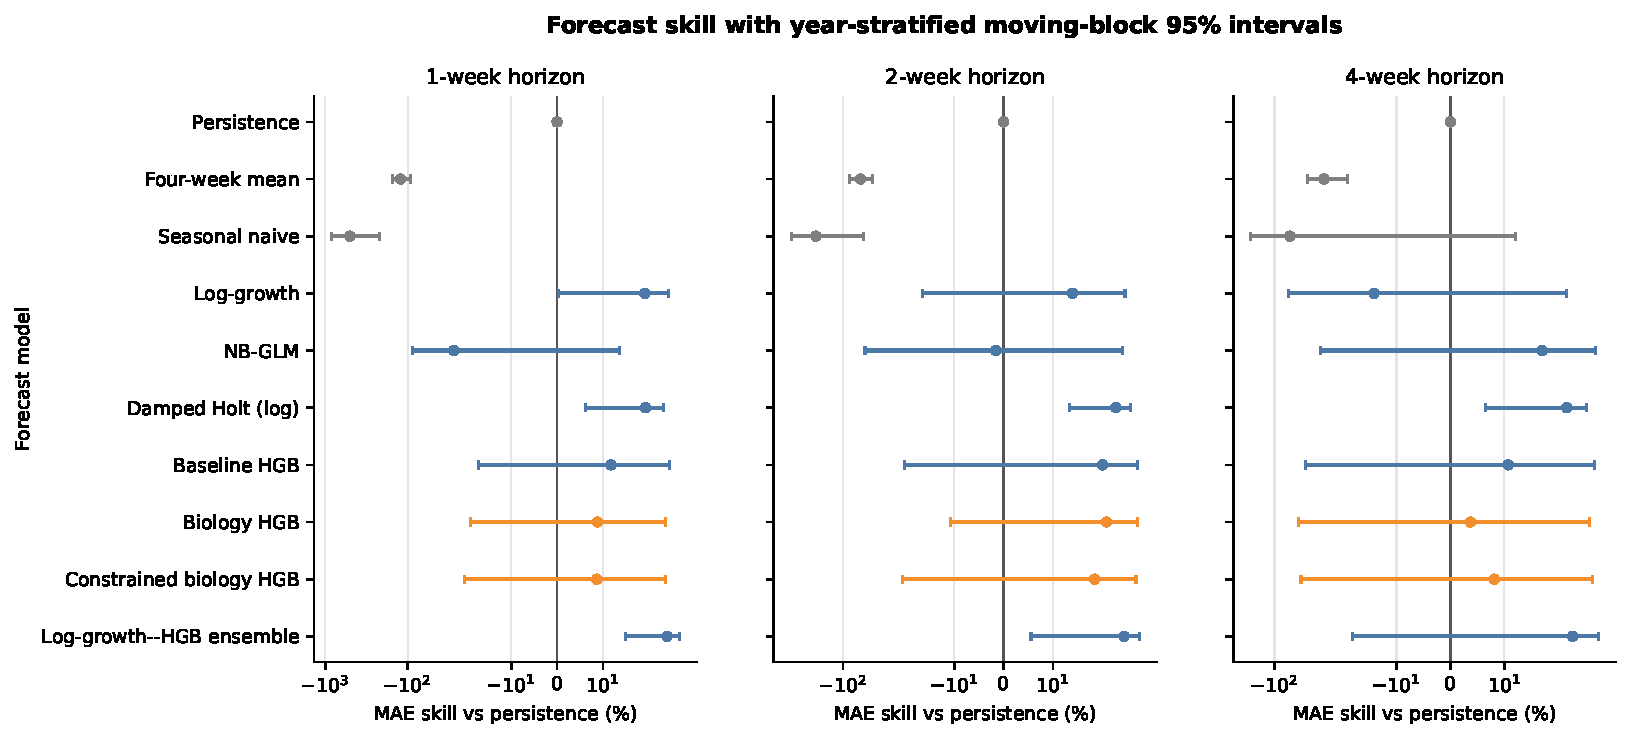
\includegraphics[width=0.90\textwidth]{forecast_performance.pdf}
\caption{MAE skill relative to persistence for all primary models. Positive values indicate lower MAE than persistence; whiskers are paired year-stratified moving-block 95\% intervals.}
\label{fig:performance}
\end{figure}

\begin{table}[p]
\centering
\caption{Complete primary-model forecast comparison.}
\label{tab:forecastfull}
\scriptsize
\resizebox{\textwidth}{!}{%
\begin{tabular}{@{}rlrrrrrrrrrrr@{}}
\toprule
$h$ & Model & $N$ & MAE & RMSE & WAPE & Bias & Peak MAE & Skill (\%) & Coverage (\%) & Width & Interval score \\
\midrule
\tableinput{tables/forecast_full.tex}
\bottomrule
\end{tabular}}
\begin{minipage}{0.98\textwidth}
\footnotesize\emph{Note:} Skill is the percentage MAE reduction relative to persistence at the same horizon. Coverage, width, and interval score refer to nominal 80\% sequential planning intervals. Damped Holt has fewer targets because it requires a contiguous observed training segment; no missing outcome was filled to increase its sample.
\end{minipage}
\end{table}
\clearpage

\subsection{Joint national forecast and divisional allocation}

Across \JointWeeks\ matched weeks, ensemble point forecasts with pooled recent shares produced 14.5\% unweighted mean shortage, 11.1\% admissions-weighted shortage, and 307.3 admission-equivalent shortfalls per week (31,033 in total); unused allocation averaged 11.5\%, and every division was covered in 6.9\% of weeks (Table~\ref{tab:allocation}). Total allocated units were 96.8\% of total observed divisional admissions. The observed-total oracle with the same shares produced 8.9\% mean shortage and 136.6 shortfalls per week. The paired oracle gap was 5.67 percentage points (95\% moving-block interval 3.08--8.36), showing that national forecast and aggregation mismatch made a material contribution beyond spatial-share error.

\begin{table}[H]
\centering
\caption{Joint forecast--allocation results over \JointWeeks\ target weeks.}
\label{tab:allocation}
\scriptsize
\resizebox{\textwidth}{!}{%
\begin{tabular}{@{}lrrrrrrr@{}}
\toprule
Strategy & Mean shortage & Weighted shortage & Mean shortfall & P90 shortage & Unused & Total budget/total observed & Full coverage \\
 & (\%) & (\%) & (admissions/week) & (\%) & (\%) & (\%) & (\%) \\
\midrule
\tableinput{tables/allocation_primary.tex}
\bottomrule
\end{tabular}}
\begin{minipage}{0.98\textwidth}
\footnotesize\emph{Note:} ``Weighted shortage'' equals total shortfall divided by total reported admissions. The primary budget measure is total allocated admission-equivalents divided by total observed admissions across all weeks; it is not the mean of weekly ratios.
\end{minipage}
\end{table}

The point policy's mean weekly budget/actual ratio was 106.2\%, whereas the primary ratio of aggregate allocated units to aggregate observed admissions was 96.8\%. High ratios in low-volume weeks receive equal weight in the former. In addition, the published divisional totals were 4.5\% higher in aggregate than the matched daily national totals, so the budget ratio should not be interpreted as pure under- or overforecasting.

Allocation conclusions were not an artifact of using only the retrospectively best forecast (Table~\ref{tab:forecastchoice}). With pooled shares, baseline HGB produced 16.2\% mean shortage, 15.2\% weighted shortage, and 419.3 shortfalls per week; the prospective rolling selector produced 14.9\%, 12.0\%, and 331.5, respectively, compared with 14.5\%, 11.1\%, and 307.3 for the ensemble. Direct divisional log-growth forecasts produced 13.4\% mean and 8.5\% weighted shortage over 99 eligible weeks, but used a materially larger aggregate budget (109.6\% of observed admissions versus 96.8\% for ensemble plus pooled shares), so their lower shortage is not a budget-matched superiority claim.

\begin{table}[H]
\centering
\caption{Allocation sensitivity to national forecast choice and direct divisional forecasting.}
\label{tab:forecastchoice}
\scriptsize
\resizebox{\textwidth}{!}{%
\begin{tabular}{@{}llrrrrrr@{}}
\toprule
Forecast & Spatial rule & $N$ & Mean shortage (\%) & Weighted shortage (\%) & Mean shortfall/week & Total budget/total observed (\%) & Unused (\%) \\
\midrule
\tableinput{tables/forecast_choice_sensitivity.tex}
\bottomrule
\end{tabular}}
\begin{minipage}{0.98\textwidth}
\footnotesize\emph{Note:} National models use the same 101 target weeks. Direct divisional log-growth requires four prior within-year observations and therefore has 99 targets. Rows are descriptive at their realized budgets, not mutually budget-matched.
\end{minipage}
\end{table}

Fixed uplifts traced a monotone mean shortage--unused allocation frontier (Table~\ref{tab:reserve}; Figure~\ref{fig:frontier}). A 20\% reserve reduced mean weekly shortage from 14.5\% to 8.6\%, admissions-weighted shortage from 11.1\% to 4.6\%, and mean absolute shortfall from 307.3 to 127.0 admissions per week, while increasing unused allocation from 11.5\% to 19.8\%. Its aggregate budget ratio was 116.1\%. The curve is a choice set, not evidence that 20\% or any other reserve is optimal.

\begin{table}[H]
\centering
\caption{Fixed-reserve points above the one-week national point forecast.}
\label{tab:reserve}
\resizebox{\textwidth}{!}{%
\begin{tabular}{@{}rrrrrrr@{}}
\toprule
Reserve & Mean shortage & Weighted shortage & Surge shortage & Mean shortfall/week & Unused & Total budget/total observed \\
(\%) & (\%) & (\%) & (\%) & (admissions) & (\%) & (\%) \\
\midrule
\tableinput{tables/fixed_reserve_frontier.tex}
\bottomrule
\end{tabular}}
\end{table}

\begin{figure}[H]
\centering
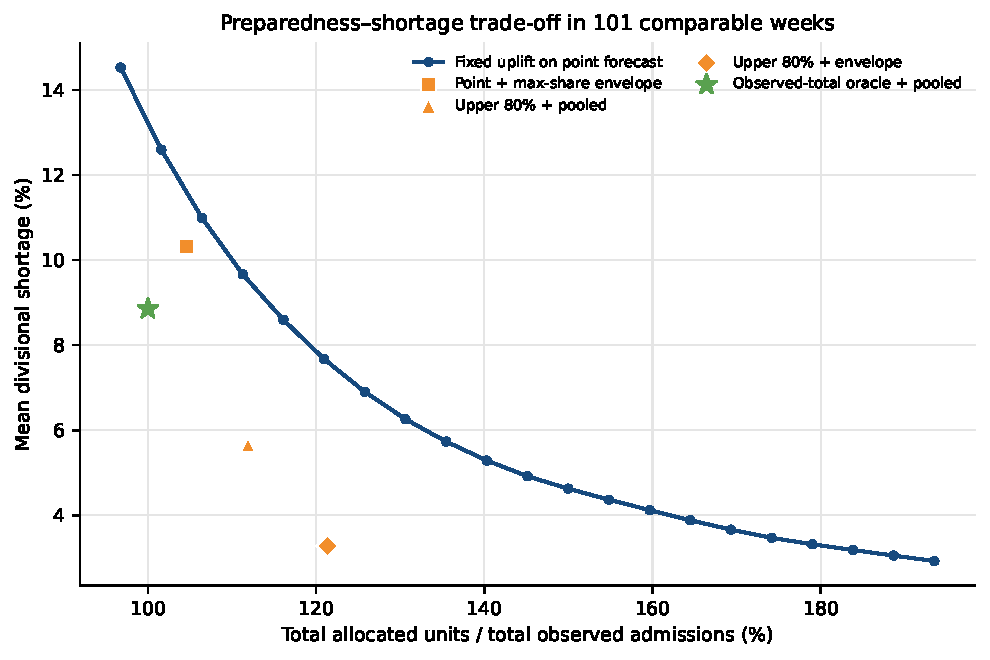
\includegraphics[width=0.88\textwidth]{allocation_frontier.pdf}
\caption{Preparedness frontier for fixed national reserves, with adaptive policies shown at their realized aggregate budgets. The horizontal axis is total allocated units divided by total observed admissions. Lower shortage requires more unused allocation; no point is labeled optimal without a cost function.}
\label{fig:frontier}
\end{figure}

Exact aggregate-budget matching changed the interpretation of adaptive policies (Table~\ref{tab:matched}). All three adaptive rules reduced unweighted mean shortage relative to their fixed comparators: by 1.24 percentage points for the point max-share envelope, 3.85 for upper-bound pooled shares, and 4.33 for the upper-bound envelope; all corresponding 95\% intervals excluded zero. Admissions-weighted differences were much smaller and uncertain: $+0.24$, $-0.29$, and $-0.71$ percentage points, respectively, with all intervals crossing zero. On surge weeks, upper-bound pooled shares were worse than the aggregate-budget-matched fixed rule by 0.76 points (95\% interval 0.28--1.24); the other surge intervals crossed zero. Adaptive timing therefore helped the average week, but evidence of benefit for high-volume admissions was absent.

\begin{table}[H]
\centering
\caption{Adaptive policies compared with exact aggregate-budget-matched fixed reserves.}
\label{tab:matched}
\scriptsize
\resizebox{\textwidth}{!}{%
\begin{tabular}{@{}lrrrrrrrr@{}}
\toprule
Adaptive policy & Matched fixed uplift (\%) & $\Delta$ mean (pp) & 95\% interval & $\Delta$ weighted (pp) & 95\% interval & $\Delta$ surge (pp) & 95\% interval & $\Delta$ unused (pp) \\
\midrule
\tableinput{tables/budget_matched.tex}
\bottomrule
\end{tabular}}
\begin{minipage}{0.98\textwidth}
\footnotesize\emph{Note:} Fixed comparators exactly match each adaptive policy's ratio of total allocated units to total observed admissions. Differences are adaptive minus matched fixed. Positive shortage values favor the fixed reserve. Intervals are year-stratified four-week moving-block bootstrap 95\% intervals.
\end{minipage}
\end{table}

\subsection{Partial identification under potentially capacity-censored surveillance}

The stress test covered 10 spatial profiles, four maximum latent-demand uplifts, five reserve levels, and four policies. Figure~\ref{fig:censoring} shows how the capacity-proxy policy changed mean shortage relative to pooled reported shares. Gains occurred under some assumptions, particularly when hidden demand was constructed to resemble the proxy, but they did not generalize across misspecified spatial patterns.

Decision-aligned minimax proxy weights varied with both latent uplift and national reserve; selected weights included 0, 0.25, 0.40, 0.65, 0.80, and 1.00. There was therefore no stable evidence supporting one capacity-proxy weight as an operational rule. A descriptive plateau check found 10 adjacent top-decile high-to-high transitions, three of which changed by no more than 5\%, but this cannot distinguish saturation from epidemic dynamics, reporting practice, or chance. The stress test bounds consequences conditional on assumptions; it does not establish that censoring occurred or estimate unmet demand.

\begin{figure}[H]
\centering
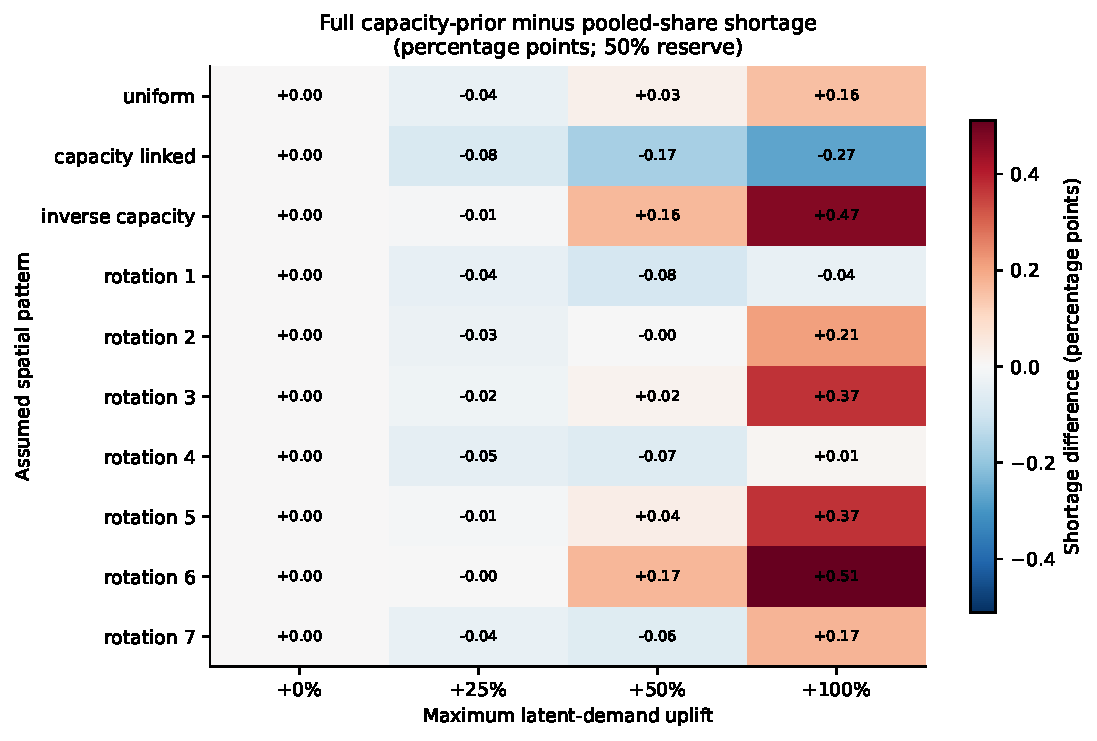
\includegraphics[width=0.90\textwidth]{censoring_robustness.pdf}
\caption{Difference in mean shortage between annual-occupancy-proxy and pooled-share allocation across latent-demand profiles and reserve levels. Negative values favor the proxy; sensitivity to the assumed profile precludes a stable operational recommendation.}
\label{fig:censoring}
\end{figure}

\section{Discussion}

\subsection{Principal findings}

Three findings are most important. First, weekly forecasting of reported national dengue admissions was workable at a one-week horizon. A simple equal-weight ensemble improved materially on either log-growth or HGB alone and on persistence, but it was identified from the completed hindcast. The prospective selector approached it at one and two weeks and deteriorated at four weeks. The appropriate lesson is that complementary trend extrapolation and nonlinear shrinkage can be useful, not that this fitted ensemble is a prospectively proven winner. Operational use should rely on frozen weekly forecasts, frequent updating, and continued monitoring.

Second, biology-informed constraints were scientifically reasonable but did not yield reliable accuracy gains. The distributed lags explicitly covered rainfall and temperature effects on mosquitoes followed by infection-to-hospitalization delay, answering an important mechanistic concern. Still, national capital-point weather and a simplified thermal response did not add enough information beyond recent admissions and seasonality. This negative result is useful because it limits a common overclaim: a model is not made more accurate merely by making one component biologically plausible.

Third, forecast accuracy alone did not determine allocation quality. The observed-total oracle showed that national forecast and aggregation mismatch accounted for a material part of shortage, but spatial mismatch remained even with the total known. HGB, prospective-selection, and direct-divisional sensitivities preserved the central shortage--budget trade-off. At exact aggregate-budget matches, adaptive rules improved unweighted average-week shortage but did not show a clear admissions-weighted benefit, and upper-bound pooled allocation worsened surge-week shortage. The comparison matters because an adaptive policy can appear attractive only because it spends more or shifts resources toward low-volume weeks.

\subsection{Interpretation relative to prior literature}

Our forecast findings reinforce earlier warnings that climate variables should be tested against strong seasonal and autoregressive baselines \citep{johansson2016,leung2023}. They also agree with probabilistic dengue studies showing horizon- and season-dependent performance \citep{johansson2019,colon2021}. Within Bangladesh, the study complements rather than replaces models using richer meteorological, socioeconomic, serotype, or district-level covariates \citep{dey2022,mobin2024,rahman2025,faruk2026,fuad2026}. Its distinct contribution is the validated weekly admission estimand, leakage-safe missing-data rules, explicit negative biological result, and decision-linked scoring.

The allocation results parallel the central argument of allocation scoring rules: a forecast should be judged partly by the decisions it supports \citep{gerding2024}. Unlike optimization studies with observed capacity and costs, however, the present data cannot identify a physical optimum. Reporting a reserve frontier and exact aggregate-budget-matched comparisons is therefore more defensible than attaching an unsupported objective function to missing capacity variables. Similarly, partial identification is preferable to treating annual all-cause occupancy as though it measured current dengue bed availability.

\subsection{What reported admissions can and cannot support}

Incomplete admission data weakens claims about population incidence and total clinical need, but it does not invalidate forecasting the workload reported by participating facilities. The more serious problem is endogenous censoring: when beds bind, admissions may stop rising even if eligible demand continues. A forecast trained on admissions could then predict the constrained observation process rather than unconstrained need. Our scenarios expose the policy sensitivity but cannot identify the hidden quantity. Accordingly, all results are stated in reported-admission or admission-service-equivalent units.

Beds are the closest next resource because a length-of-stay distribution converts admissions into bed occupancy. Even so, exact occupied beds require daily admission and discharge timestamps plus staffed capacity. Intravenous-fluid procurement additionally requires clinical mix, opening inventory, receipts, issues, wastage, stockouts, and lead times. Physician and nurse requirements require workload standards and available shift hours; the WHO Workload Indicators of Staffing Need framework is appropriate once those data exist \citep{whoWisn}. The current work is a preparedness analysis, not a staffing norm or purchase order.

\subsection{Limitations}

The study has important limitations. Only three evaluation seasons were available, with no external geographic validation. The public outcome may omit non-hospitalized, unreported, refused, diverted, waitlisted, or transferred patients, and reporting definitions may change. Pre-2024 high-frequency history contains structural gaps, particularly in 2020--2021. NASA POWER points at divisional capitals do not measure population-weighted exposure, local water storage, or microclimate. Biological features omit vector abundance, serotype, immunity, mobility, and interventions.

The best-in-backtest ensemble was identified using the completed hindcast; its rolling-selector sensitivity and a future frozen season are therefore essential checks against selection optimism. Sequential interval coverage is empirical under temporal dependence rather than an exact exchangeability guarantee. The direct divisional baseline had two fewer weeks and a different realized budget, so it is not a causal comparison. Published divisional and daily national totals differ, complicating budget interpretation. The annual all-cause occupancy proxy is temporally and clinically misaligned. Clinical conversion coefficients come from a selected Group B/C cohort in three Dhaka hospitals. Finally, no verified resource cost, inventory, transfer, or staff-availability data were available, so the study cannot estimate a cost-optimal or physically feasible hospital allocation.

\subsection{Prospective validation and next data}

The highest-value follow-on dataset is one or more outbreak seasons from sentinel hospitals, recorded daily: total suspected and confirmed dengue presentations; admitted patients; refusals for no bed, diversions, waitlists, and transfers; staffed and occupied dengue beds; and admission and discharge timestamps. These fields would identify the presentation-to-admission observation process and allow direct occupancy validation. Facility inventory movements, delivery lead times, and workforce hours could then support multi-resource optimization.

A prospective protocol should freeze each forecast before the target week, archive revisions, predefine alert and reserve thresholds, and score both forecast and decision outcomes. Candidate outcomes include shortage, unused reserve, transfers, waiting time, worst-site service, stockouts, and cost. Such data would support a stronger subsequent study of unmet demand and facility-constrained allocation rather than serving as a minor patch to the present admissions-based analysis.

\section{Conclusion}

A useful one-week forecast of reported dengue admissions in Bangladesh is feasible with conservative missing-data rules and repeated historical-origin evaluation. An equal-weight log-growth--HGB ensemble performed best in the completed hindcast, while a prior-origin-only selector provided a more realistic prospective sensitivity. Biologically informed weather features and constraints did not reliably improve accuracy. The negative biological result should be retained because it tests, rather than assumes, the value of scientific structure.

For resource planning, fixed reserves provide a transparent benchmark that adaptive policies must beat at the same ratio of total allocated units to total observed admissions. The observed-total oracle, forecast-choice and direct-divisional baselines, aggregate-budget-matched comparisons, and latent-demand scenarios show where forecast error, spatial instability, and unobserved need enter the decision. With current public data, the defensible output is a shortage--reserve frontier under potentially capacity-censored surveillance. Facility-level presentations, admissions, denied or displaced demand, staffed occupancy, timestamps, inventory, and workforce data are required before claiming exact beds, fluids, doctors, nurses, or an optimal allocation.

\section*{Declarations}

\textbf{Ethics approval and consent to participate.} Ethics approval and consent to participate were not required because this study analyzed only publicly accessible, aggregate, non-identifiable surveillance and environmental data and involved no participant recruitment, intervention, or access to individual records.

\textbf{Data and code availability.} The reproducibility package accompanying this manuscript contains the public-source registry, cached aggregate inputs used for the frozen analysis, processed data, machine-readable results, scripts, figures, tables, and LaTeX source. GitHub repository: \texttt{INSERT-GITHUB-URL-HERE}. Zenodo archive and DOI: \texttt{INSERT-ZENODO-DOI-OR-URL-HERE}. Third-party data remain subject to their original terms.

\textbf{Funding.} This research did not receive any specific grant from funding agencies in the public, commercial, or not-for-profit sectors.

\textbf{Declaration of competing interest.} The authors declare that they have no known competing financial interests or personal relationships that could have appeared to influence the work reported in this article.

\textbf{Author contributions (CRediT).} Abid Shahriyar: Conceptualization, Data curation, Formal analysis, Investigation, Methodology, Project administration, Resources, Software, Supervision, Validation, Visualization, Writing -- original draft, Writing -- review \& editing. Farzana Momtaz Mithila: Conceptualization, Data curation, Formal analysis, Investigation, Methodology, Project administration, Resources, Software, Supervision, Validation, Visualization, Writing -- original draft, Writing -- review \& editing.

\textbf{Clinical-use disclaimer.} Resource conversions and allocation units are research scenarios. They are not patient-level clinical guidance, procurement orders, or minimum staffing standards.

\appendix
\counterwithin{table}{section}
\counterwithin{figure}{section}
\counterwithin{equation}{section}

\section{Calendar validation and information cutoff}

For a date $d$, the weekly start is the preceding Sunday and the end is six days later. Week 1 begins on the Sunday preceding or equal to 1 January. At year boundaries, week-year is assigned consistently with the reporting interval. Automated tests retain 9--15 August 2026 as week 33. For the current illustrative forecast, 4--10 October 2026 was a complete seven-day origin week and the 11--17 October target was generated after that origin closed; a later partial target observation was not an input.

\section{Latent-demand scenario definitions}

Table~\ref{tab:scenarios} defines the complete set of latent-demand profiles used in the partial-identification analysis.

\begin{table}[H]
\centering
\caption{Partial-identification grid for potentially unobserved admission-eligible demand.}
\label{tab:scenarios}
\small
\begin{tabularx}{\textwidth}{@{}p{0.20\textwidth}X p{0.23\textwidth}@{}}
\toprule
Profile & Definition & Purpose \\
\midrule
Uniform & Equal proportional uplift in all eight divisions & Changes total demand without altering spatial shares \\
Capacity-linked & Uplift increases with normalized annual all-cause occupancy & Assumption most favorable to the proxy \\
Inverse capacity & Uplift decreases with the occupancy proxy & Direct spatial misspecification test \\
Rotations 1--7 & Capacity-linked score shifted across one to seven division positions & Seven systematic misspecification patterns preserving the score distribution \\
\bottomrule
\end{tabularx}
\begin{minipage}{0.95\textwidth}
\footnotesize\emph{Grid:} four maximum uplifts (0, 25, 50, 100\%) $\times$ five reserve levels (0, 25, 50, 75, 100\%) $\times$ four policies $\times$ ten profiles = 800 profile-level combinations and 80,800 week-policy observations over 101 weeks.
\end{minipage}
\end{table}

\section{Illustrative resource conversion}

At the frozen 4--10 October 2026 origin, the one-week forecast for 11--17 October was \OneWeekForecast\ reported admissions, with an 80\% planning interval of \OneWeekLower--\OneWeekUpper. A deliberately conservative illustration uses the upper bound plus 25\% latent-demand sensitivity, or approximately 19,393 planning admissions. Applying the selected cohort's five-day stay produces approximately 96,965 bed-days (13,852 average occupied-bed equivalents during a seven-day week). Applying 4.5 L per admission produces approximately 87,270 L, or 174,540 half-liter equivalents.

These are not minimum orders. The latent uplift is not estimated, patient acuity and fluid treatment vary, opening stock is unknown, and cohort medians are not national parameters. A facility occupancy model should convolve daily arrivals with a length-of-stay distribution. A procurement model must subtract usable stock and scheduled receipts and incorporate lead time, wastage, stockouts, and package sizes.

\section*{Declaration of generative AI and AI-assisted technologies in the manuscript preparation process}

During the preparation of this work, the authors used OpenAI Codex to assist with checking journal-formatting requirements, reference links and bibliographic metadata, and with language and LaTeX editing. After using this tool, the authors reviewed and edited the content as needed and take full responsibility for the content of the published article.

\printbibliography

\end{document}
